\section{Programme}
Für alle Module wurde ein gemeinsamer Programmcode geschrieben, bei dem mithilfe von einem \#define ausgewählt wird, welche Funktionen kompiliert und auf den jeweiligen Mikrocontroller geflasht werden. Die Wichtigsten dieser Funktionen werden in den Kapiteln \ref{Modulübergreifende Funktionen} bis \ref{Code der Eingabemodule} näher erläutert. Diese Herangehensweise wurde gewählt, da bei der Programmierung größerer Mengen von Mikrocontrollern die Wahrscheinlichkeit hoch ist, falsche Software zu flashen, wenn es mehrere sehr ähnliche Programme gibt. Zusätzlich ist die Entwicklung neuer Funktionen deutlich einfacher, da eine für alle Module notwendige Änderung nicht in mehrere Quelldateien angepasst werden muss.

\section{Modulübergreifende Funktionen}
\label{Modulübergreifende Funktionen}
Die Funktionen zum Lesen und Senden von Nachrichten müssen auf allen Modulen implementiert werden.

\subsection{Senden einer Nachricht}
Um eine Nachricht auf den Bus zu schreiben, muss zunächst festgestellt werden, dass dieser gerade nicht beschrieben wird. Nur, wenn dies der Fall ist, kann die Nachricht gesendet werden.	Die Nachricht setzt sich aus den in Kapitel \ref{Datenbus} beschriebenen Teilen zusammen. Jedes dieser Teile wurde als eigenen Funktion implementiert und schlussendlich in einer übergreifenden Funktion zusammengeführt.

\lstinputlisting[firstline= 240, lastline=250,language = C++,frame=single,label=send(),caption=Senden einer Nachricht]{
	Kapitel/Programme/main.cpp}


\subsection{Empfangen einer Nachricht}
Solange ein Modul keine Nachricht senden möchte, hört es auf die Kommunikation auf dem Bus. Bei jedem empfangenen Start of Frame wird die Busfrequenz berechnet und gespeichert. Wenn die empfangene Adresse mit der eigenen Adresse übereinstimmt, wird der restliche Teil der Nachricht empfangen, gespeichert und zur weiteren Verarbeitung vorbereitet. Auch in diesem Fall wurde jeder Abschnitt der Nachricht als separate Funktion implementiert und anschließend in einer übergreifenden Funktion zusammengeführt.\\

\lstinputlisting[firstline= 139, lastline=148,language = C++,frame=single,label=recieve(),caption=Empfangen einer Nachricht]{
	Kapitel/Programme/main.cpp}

\section{Hauptmodul - Programmcode}
Das Hauptmodul übernimmt die folgenden Aufgaben:
\begin{enumerate}
    \item Verwaltung der Adressvergabe an angeschlossene Module
    \item Abfrage nach neuen Daten der einzelnen Module
    \item Übermittlung dieser Daten über eine UART-Schnittstelle an den angeschlossenen Rechner
\end{enumerate}

\begin{figure}[H]
	\centering    
	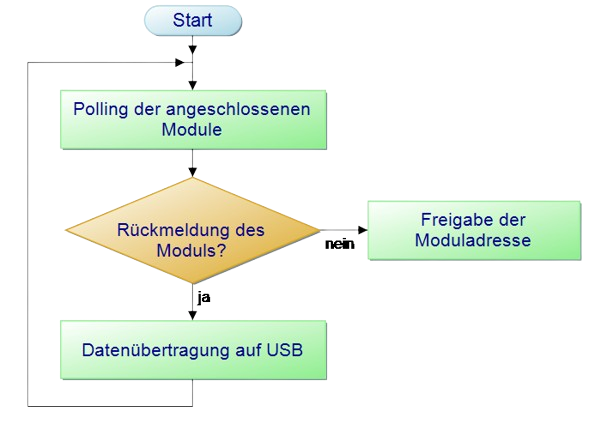
\includegraphics[width=.75\textwidth]{Bilder/pap_hauptmodul.png}
	\caption{Programmablauf Hauptmodul}
	\label{Programm_Hauptmodul}
\end{figure}
\textmd{
}

\subsection{Adressvergabe und Verwaltung}
Das Hauptmodul speichert alle vergebenen Adressen zusammen mit den zugehörigen Funktionen sowie weiteren Variablen der jeweiligen Module in einer Liste von Structs. Diese Liste wird für das Polling der Teilnehmer verwendet, wodurch sichergestellt wird, dass ausschließlich die tatsächlich angeschlossenen Module abgefragt werden.\\


\lstinputlisting[firstline= 4, lastline=20,language = C++,frame=single,label=structDevice,caption=Struct device]{Kapitel/Programme/header.h}


Die jeweiligen Module haben keine festgelegte Adresse. Wenn diese also mit Spannung versorgt werden, warten sie auf die Adressvergabe des Hauptmoduls. In der Polling Liste wird eine bestimmte Adresse abgefragt, um festzustellen, ob ein neuer Teilnehmer an den Bus angeschlossen wurde. Wenn eine Rückmeldung auf diese Adresse festgestellt wird, dann enthält die nächste Nachricht die Adresse für den neuen Teilnehmer. In der Rückmeldung eines Moduls ist dessen Funktion hinterlegt. Diese Informationen werden in der Adressliste abgespeichert und das Gerät ab dem Zeitpunkt mit abgefragt.\\

\lstinputlisting[firstline= 319, lastline=339,language = C++,frame=single,label=newAdress(),caption= Zuweisen einer neuen Adresse]{Kapitel/Programme/main.cpp}

Wenn ein Modul nicht mehr über den Bus kommuniziert, wird dessen Adresse nach mehreren fehlgeschlagenen Versuchen (Timeout) aus der Polling-Liste entfernt und wieder den verfügbaren Adressen zugewiesen. Dadurch wird sichergestellt, dass alle aktiven Geräte schnellstmöglich vom Hauptmodul abgefragt werden und Adressen für neu verbundene Geräte freigegeben werden.
\\

\lstinputlisting[firstline= 395, lastline=424,language = C++,frame=single,label=timeout(),caption=Timeout Funktion]{Kapitel/Programme/main.cpp}

Wenn keine Antwort eines Eingabemoduls in der vorgegebenen Wartezeit empfangen wird, wird der Timeout-Counter iteriert. Sobald dieser seinen Maximalwert erreicht, wird das Gerät nicht mehr abgefragt und dessen Adresse freigegeben.


\subsection{Abfrage neuer Daten}
Die Daten jedes Moduls werden einmal pro Durchlauf der Polling Liste abgefragt. Sobald neue Daten empfangen wurden, werden diese abgespeichert und dem angeschlossenen Computer über die UART-Schnittstelle übermittelt.\\

\lstinputlisting[firstline= 426, lastline=459,language = C++,frame=single,label=polling(),caption=Polling Funktion]{
	Kapitel/Programme/main.cpp}

\subsection{Übermittlung der Daten an den angeschlossenen Computer}
Sobald neue Daten von einem Modul empfangen worden sind, werden diese an den Computer übermittelt. Diese Kommunikation erfolgt über eine UART Schnittstelle und den auf dem PCB verbauten UART zu USB Bridge IC. Zu den übermittelten Daten wird neben der jeweiligen Funktion auch die zugehörige Adresse übermittelt, sodass die Daten nicht nur abhängig von der Funktion ausgewertet werden können, sondern auch mehrere gleiche Module voneinander unterschieden werden können.\\


\lstinputlisting[firstline= 304, lastline=310,language = C++,frame=single,label=usb(),caption=Datenübertragung an den angeschlossenen Computer]{
	Kapitel/Programme/main.cpp}


\section{Code der Eingabemodule}
\label{Code der Eingabemodule}
Im Folgendem wird der Programm-Ablauf eines Eingabemoduls genauer beschrieben. Dieses Modul hat folgende Aufgaben:
\begin{enumerate}
    \item Anforderung einer Adresse bei Neustart
    \item Auswerten der Modulfunktion
    \item Übermitteln der Daten an das Hauptmodul bei Anfrage
\end{enumerate}

\begin{figure}[H]
	\centering    
	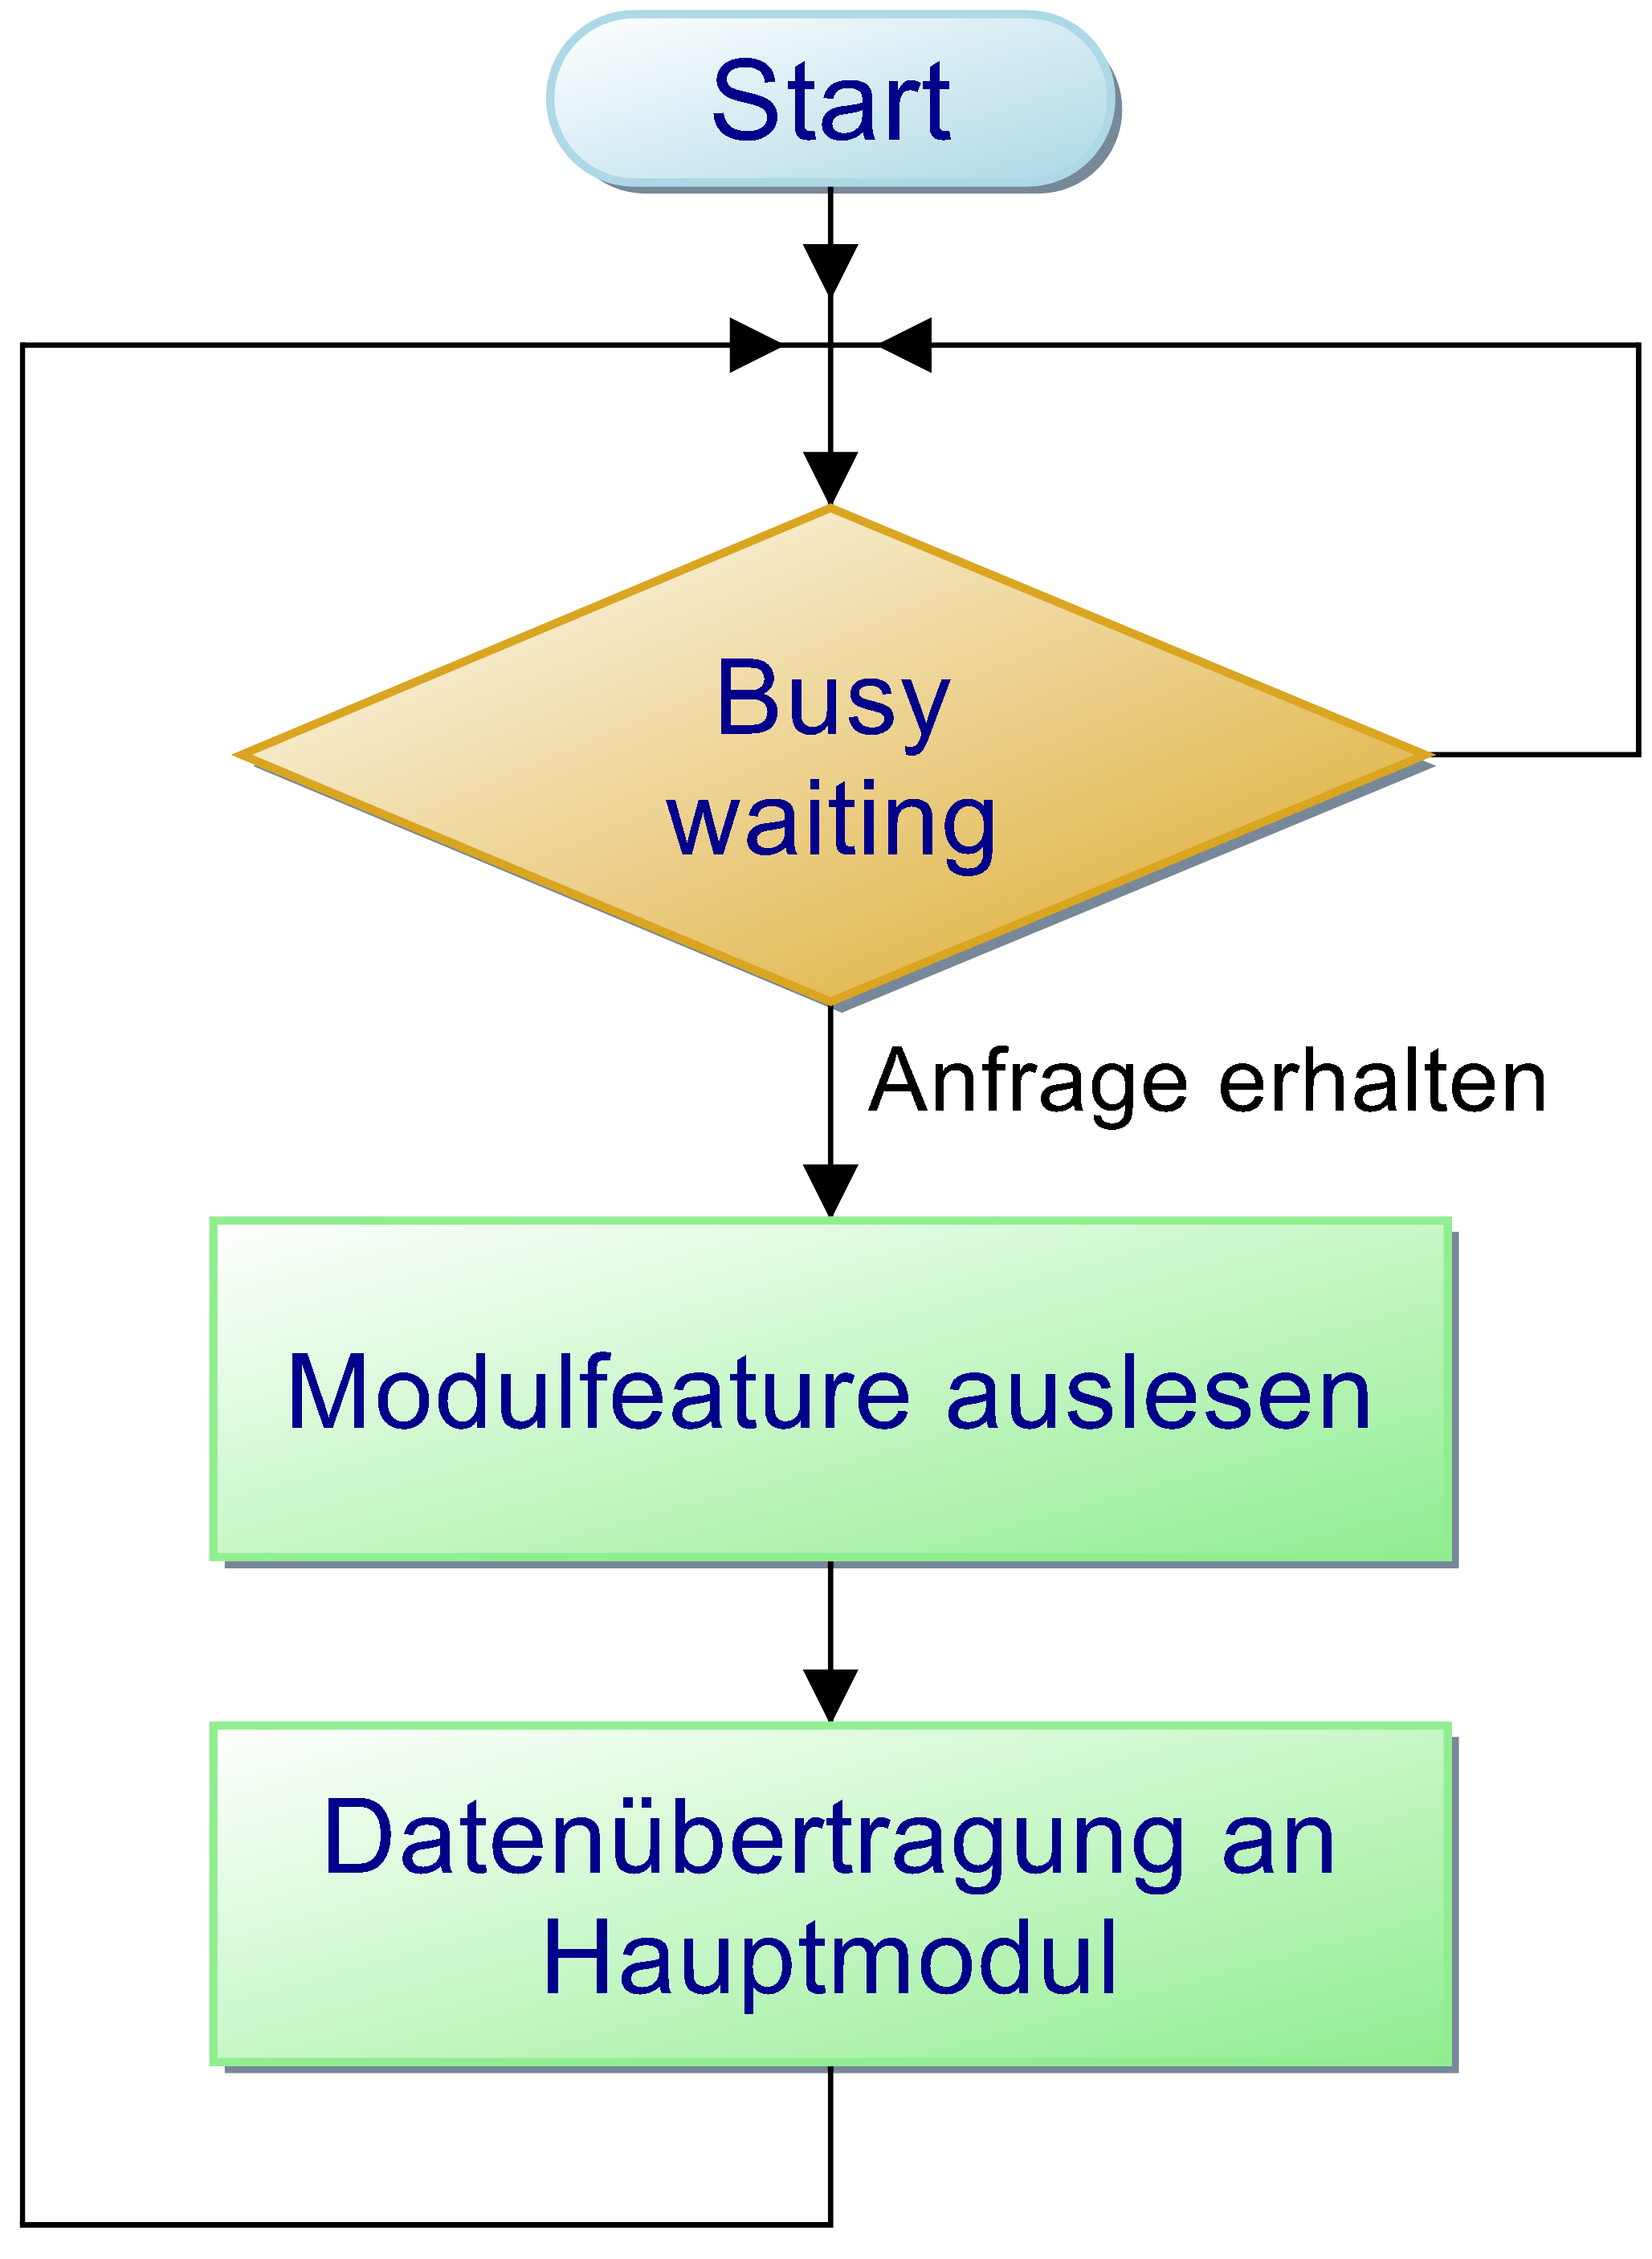
\includegraphics[width=.75\textwidth]{Bilder/pap_eingabemodul.png}
	\caption{Programmablauf eines Eingabemoduls}
	\label{Programm_Eingabemodul}
\end{figure}


\subsection{Anforderung einer Adresse}
Wenn einem Modul noch keine Adresse zugewiesen wurde und der Kontroller nach neuen Teilnehmern auf dem Bus sucht, antwortet das Modul mit einer Nachricht, in der seine Funktion in den übertragenen Daten enthalten ist. Anschließend übermittelt der Hauptcontroller eine neue Adresse an das Modul. Diese Adresse wird vom Modul gespeichert, sodass es danach ausschließlich auf diese Adresse reagiert.\\

\lstinputlisting[firstline= 281, lastline=290,language = C++,frame=single,label=getAdress(),caption=Anfordern einer Adresse]{
	Kapitel/Programme/main.cpp}


\subsection{Auswertung der Modulfunktion}
Die Auswertung der Modulfunktion ist abhängig von der jeweiligen Funktion des Moduls und kann daher nicht verallgemeinert werden.\\
Im Fall des Tastatur-Moduls werden die Tasten nur dann ausgewertet, wenn der Kontroller das Modul abfragt. Anschließend werden die Daten übermittelt. Für diese Auswertung wurde eine allgemeine Funktion geschrieben, die jedoch für jedes Modul spezifisch angepasst werden muss.\\

\lstinputlisting[firstline= 292, lastline=300,language = C++,frame=single,label=myfunction(),caption=Modul abhängige Funktion]{Kapitel/Programme/main.cpp}

\subsection{Übermittlung der Daten an das Kontroller-Modul}
Sobald eine Anfrage des Hauptmoduls an die Adresse des Eingabemoduls empfangen wird, übermittelt dieses die Information der Modulfunktion. Im Falle der Tastatur wären dies die zurzeit gedrückten Tasten.

